\documentclass{article}

\usepackage{graphicx} % inserting images
\usepackage{hyperref} % hyperlinks
\hypersetup{ % hyperlink config
    colorlinks=true,
    linkcolor=blue, % equation numbers
    filecolor=magenta,      
    urlcolor=blue, % href links
    }
\usepackage{amsmath} % math formatting
\usepackage{amssymb} % math symbols

\usepackage{tikz} % render plots
\usepackage{pgfplots}
\pgfplotsset{compat=1.18}

\usepackage[many]{tcolorbox} % callout box
\usepackage{csquotes} % quotes
%\usepackage{emoji} % emoji

\pgfplotsset{compat=1.17} % render plots

\newcommand{\argmax}{\operatornamewithlimits{argmax}}
\newcommand{\argmin}{\operatornamewithlimits{argmin}}

\newcommand{\code}[1]{\texttt{\detokenize{#1}}}

\newcommand{\callouttext}[2]{\emoji{#1} \textbf{#2}\smallskip}
\newtcolorbox{callout}{
    colback = sub, 
    colframe = main, 
    boxrule = 0pt, 
    leftrule = 6pt % left rule weight
}
\newenvironment{infobox}{\wrapfigure{r}{5cm}}{\endwrapfigure}
\definecolor{main}{HTML}{5989cf}    % setting main color to be used
\definecolor{sub}{HTML}{cde4ff}     % setting sub color to be used
\tcbset{
    sharp corners,
    colback = white,
    before skip = 0.2cm,    % add extra space before the box
    after skip = 0.5cm      % add extra space after the box
}

\setlength{\parindent}{0pt} % don't indent on new paragraphs

%% Heading
\title{The Hyperdrive-Yieldspace AMM}
\author{Dylan Paiton}

%% Document
\begin{document}

\maketitle


\begin{abstract}
This document gives a complete description of the Hyperdrive + Yieldspace AMM.
In contrast to the existing \href{https://github.com/delvtech/hyperdrive/blob/main/docs/Hyperdrive_Whitepaper.pdf}{Hyperdrive whitepaper}, which provides an abstracted view of how Hyperdrive can be built on top of any AMM curve, this document provides details of the specific implementation deployed by the Element DAO on Ethereum mainnet and several L2 chains.
\end{abstract}

\section{Introduction}

\subsection{The Hyperdrive-Yieldspace AMM}

For a deployed market pool, the Hyperdrive-Yieldspace AMM uses a modified \href{https://yield.is/YieldSpace.pdf}{constant power sum formula} to derive a price relationship between two assets.
In this case, our assets are vault shares, $z$, and bonds, $y$.
When base, $x$, is supplied to the pool, it is converted into shares, $z$, by depositing the base into an underlying yield bearing vault.
The relationship between base and shares is determined via the vault share price, $c = \tfrac{x}{z}$.
The Hyperdrive AMM also accounts for an additional ``zeta'' adjustment to produce the effective shares, $z_e = z - \zeta$, as described in the \href{https://github.com/delvtech/hyperdrive/blob/main/docs/Hyperdrive_Whitepaper.pdf}{whitepaper}.
Finally, the AMM then mints bonds, $y$, such that $k$ is kept constant.
In accordance with the YieldSpace AMM dynamics, effective shares and bonds are related via an invariance formula:

\begin{equation}\label{keq}
k = \tfrac{c}{\mu} (\mu z_e)^{1 - t_{s}} + y^{1 - t_{s}}
\end{equation}

where $t_{s}$ is a time stretch constant that influences price slippage, and $\mu$ is the vault share price when the Hyperdrive pool was created.

\section{Shorts}
\subsection{Open short}

\subsubsection{Trader deposit}\label{trader-deposit}
For some number of bonds being shorted, $\Delta y$, the short deposit in shares is made up of several components:

\begin{itemize}
\item The \textbf{total value} that underlies the bonds: $V(\Delta y) = \left( \frac{c_1}{c_0} + \phi_f \right) \cdot \frac{\Delta y}{c}$
\item The \textbf{curve fee}: $\Phi_{\text{c,os}}(\Delta y) = \phi_{c} \cdot (1 - p) \cdot \frac{\Delta y}{c}$
\item The \textbf{short principal}: $L(\Delta y) = z_e - \tfrac{1}{\mu} \cdot (\tfrac{\mu}{c} \cdot (k - (y + \Delta y)^{1 - t_s}))^{\tfrac{1}{1 - t_s}}$
\end{itemize}

where $p$ is the \textbf{spot price}, which defines the relationship between shares and bonds when making an infinitesimally small trade and is given by

\begin{equation}\label{spot-price}
p = \left( \tfrac{\mu \cdot z_e}{y} \right)^{t_s}
\end{equation}

The trader opening a short has to pay a \textbf{deposit}, $D(\Delta y)$, which is their maximum loss when closing the short, or

\begin{equation}\label{short-deposit}
D(\Delta y) =
\begin{cases}
    V(\Delta y) - L(\Delta y) + \Phi_{c,os}(\Delta y),
      & \text{if } V(\Delta y) > L(\Delta y) - \Phi_{c,os}(\Delta y) \\
    0,              & \text{otherwise}
\end{cases}
\end{equation}

The cases avoid situations with negative interest and thus ensure we are trading in a valid regime.
The success case is also defined as the \textbf{short proceeds}, which are the proceeds in shares of closing a short position and are given by

\begin{equation}\label{short-proceeds}
\text{short\_proceeds} = V(\Delta y) - \Delta z = \left( \tfrac{c_1}{c_0} + \phi_f \right) \cdot \tfrac{\Delta y}{c} - \Delta z
\end{equation}

Where $\Delta z = L(\Delta y) - \Phi_{c,os}(\Delta y)$ is the fee-adjusted share delta.
Importantly, this surfaces a constraint that the short principal must be greater than the curve fee for a given $\Delta y$.
Due to the different scaling properties between the non-linear $L(\Delta y)$ and linear $\Phi_{c,os}(\Delta y)$, this constraint is not strictly a function of market parameters, but is also a function of the magnitude of $\Delta y$.

For some deposit, the realized price for the trader is

\begin{equation}\label{realized-price}
p_r = 1 - \frac{D(\Delta y)}{\Delta y}
\end{equation}

LPs take the opposite side of trades, so when a trader opens a short the LP opens a long.
The short principal is the price paid by the LP to buy bonds, which are then set aside as if ``sold'' by the trader when they opened their short.
The price the LP paid is

\begin{equation}\label{lp-price}
p_{l} = \frac{L(\Delta y)}{\Delta y}
\end{equation}

\subsubsection{Open Short Derivatives}

\subsubsubsection{Curve fee}
The curve fee derivative is:

\begin{equation}\label{curve-fee-derivative}
\Phi^{\prime}_{\text{c,os}}(\Delta y) = \tfrac{1}{c} \cdot \phi_{c} \cdot (1 - p)
\end{equation}

\subsubsubsection{Total value}
The total value derivative is also a constant:

\begin{equation}
V^{\prime}(\Delta y) = \tfrac{c_{1}}{c_{0} \cdot c} + \tfrac{\phi_{f}}{c}
\end{equation}

\subsubsubsection{Short principal}\label{short-principal-derivative}
For the short principal derivative, let:

\begin{equation}
u = \frac{\mu}{c} \cdot \left( k - (y + \Delta y)^{1-t_s} \right)
\end{equation}

\begin{equation}
\frac{du}{d \Delta y} = \frac{\mu}{c} \cdot -(1 - t_s) \cdot (y + \Delta y)^{-t_s}
\end{equation}

therefore,

\begin{equation}\label{eq-short-principal-derivative}
\begin{aligned}
L^{\prime}(\Delta y) &= - \frac{1}{\mu} \cdot \frac{1}{1-t_s} \cdot u^{\frac{1}{1-t_s} - 1} \cdot \frac{du}{d \Delta y} \\
&= - \frac{1}{\mu} \cdot \frac{1}{1-t_s} \left( \frac{\mu}{c} \left( k - (y + \Delta y)^{1 - t_s} \right) \right)^{\frac{t_s}{1-t_s}}
\cdot \frac{\mu}{c} \cdot -(1 - t_s) \cdot (y + \Delta y)^{t_s} \\
&= \frac{1}{c} \cdot (y + \Delta y)^{-t_s} \cdot \left( \frac{\mu}{c} \cdot \left( k - (y + \Delta y)^{1 - t_s} \right) \right)^{\frac{t_s}{1 - t_s}}
\end{aligned}
\end{equation}

\subsubsubsection{Short deposit}
Together these give us the short deposit derivative in units of base:

\begin{equation}
D^{\prime}(\Delta y) =
\begin{cases}
    c \cdot \left( V^{\prime}(\Delta y) - L^{\prime}(\Delta y) + \Phi^{\prime}_{\text{c,os}}(\Delta y) \right),
    & \text{if } V(\Delta y) > L(\Delta y) - \Phi_{\text{c,os}}(\Delta y) \\
    0,              & \text{otherwise}
\end{cases}
\end{equation}

Simplifying the condition where the derivative is non-zero, let:

\begin{displaymath}
\begin{aligned}
d &= c \cdot \left( V^{\prime}(\Delta y) - L^{\prime}(\Delta y) + \Phi^{\prime}_{\text{c,os}}(\Delta y) \right) \\
&= c \cdot \left( 
\left( \tfrac{c_{1}}{c_{0} \cdot c} + \tfrac{\phi_{f}}{c} \right)
- \left( \frac{1}{c} \left( \frac{\mu}{c} \cdot \left( k - (y + \Delta y)^{1 - t_s} \right) \right)^{\frac{t_s}{1 - t_s}} \cdot (y + \Delta y)^{-t_s} \right)
+ \left( \phi_{c} \cdot (1 - p) \right) \right) \\
&= 
\tfrac{c_{1}}{c_{0}} + \phi_{f}
- \left( \frac{\mu}{c} \cdot \left( k - (y + \Delta y)^{1 - t_s} \right) \right)^{\frac{t_s}{1 - t_s}} \cdot (y + \Delta y)^{-t_s}
+ c \cdot \phi_{c} \cdot (1 - p) \\
\end{aligned}
\end{displaymath}


\subsubsection{Estimating the maximum possible short}

We must compute the maximum possible short for a given pool in order to provide an upper bound for user trades.

\subsubsubsection{Share reserves after a short}
When a short trade for $\Delta y$ bonds is executed, the Hyperdrive pool's share reserves become:

\begin{equation}\label{reserve-after-max}
    z_1(\Delta y) = \tfrac{1}{\mu}
    \cdot \left( \tfrac{\mu}{c} \cdot \left( k - (y_0 + \Delta y)^{1 - t_s} \right) \right)^{\tfrac{1}{1 - t_s}}
    + \phi_c \cdot (1 - p) \cdot (1 - \phi_g) \cdot \tfrac{\Delta y}{c}
\end{equation}

We will label the left-hand side of the equation as the YieldSpace component and the right-hand side as the fee component.
The final reserve levels for bonds, $y_1 = y_0 + \Delta y$, and shares, $z_1 = z_0 + \Delta z$, result in a net increase in bonds.
The shares typically decrease, but in situations with low spot price and high fees, it is possible that the reduction in shares used to mint bonds is less than the additional shares paid by the trader in the form of fees, resulting in a net increase in pool share reserves.

\subsubsubsection{Minimum share reserves given exposure}

A pool's realized minimum share reserves is a function of the preset minimum constant, $z_{\text{min}}$, the exposure, $e$, and the share adjustment, $\zeta$:

\begin{equation}\label{solvency-constraints}
\begin{aligned}
    z_1 &\ge z_{\text{min}} \\
    z_1 &\ge z_{\text{min}} + \zeta \\
    z_1 &\ge z_{\text{min}} + \tfrac{e}{c}
\end{aligned}
\end{equation}

Exposure is a positive value represented in bonds, which we convert to shares by dividing by the vault share price.
These checks are performed independently, and thus can be combined via max operations: $ z_1 - \text{max}\left( \zeta, \tfrac{e}{c}, 0 \right) \ge z_{\text{min}}$.
When a short is opened, the exposure is reduced by the short bond amount, which impacts the solvency constraint.
To account for this, we can define the exposure after a short, $e_s(\Delta y) = \text{max}(e - \Delta y, 0)$.
With this in mind, our solvency-constrained maximum short is given by:

\begin{equation}\label{pool-min-share-reserves}
\begin{aligned}
    z_{1,\text{min}} = &z_{\text{min}} + \text{max}\left( \zeta, \tfrac{e_s(\Delta y_{\text{max}})}{c}, 0 \right) \\
    = &\tfrac{1}{\mu} \cdot \left(
    \tfrac{\mu}{c} \cdot \left( k - (y_0 + \Delta y_{\text{max}})^{1 - t_s} \right)
    \right)^{\tfrac{1}{1 - t_s}} \\
    &+ \phi_c \cdot (1 - p) \cdot (1 - \phi_g) \cdot \tfrac{\Delta y_{\text{max}}}{c}
\end{aligned}
\end{equation}


From here, we cannot determine a closed-form solution for $\Delta y_{\text{max}}$, but we can approximate it with a linear estimate.

\subsubsubsection{Conservative YieldSpace estimate}

Considering \eqref{pool-min-share-reserves}, we want to compute a linear approximation that underestimates the YieldSpace component, resulting in a smaller estimated $\Delta y$.
This can be achieved via a first-order Taylor Series tangent line approximation, which always lies below the convex YieldSpace curve:

\begin{equation}
\begin{aligned}
    z_{1,ys}(\Delta y) = f(\Delta y) &= \frac{1}{\mu} \left( \frac{\mu}{c} \left( k - \left( y_0 + \Delta y \right)^{1 - t_s} \right)\right)^{\frac{1}{1 - t_s}} \\
    &\ge f(0) + f'(0) \cdot \Delta y
\end{aligned}
\end{equation}

The derivative is computed via the chain rule:

\begin{equation}
\begin{aligned}
    h(\Delta y) &= \frac{\mu}{c} \left( k - \left( y_0 + \Delta y \right)^{1 - t_s} \right) \\
    h'(\Delta y) &= - \frac{\mu}{c} \cdot (1 - t_s) \cdot (y_0 + \Delta y)^{-t_s} \\
    f(\Delta y) &= \frac{1}{\mu} \left( h(\Delta y) \right)^{\frac{1}{1-t_s}} \\
    f'(\Delta y) &= \frac{1}{\mu} \cdot \left( \frac{1}{1 - t_s} \right) \cdot h(\Delta y)^{\frac{t_s}{1 - t_s}} \cdot h'(\Delta y) \\
    &= \frac{1}{\mu} \cdot \left( \frac{1}{1 - t_s} \right) \cdot h(\Delta y)^{\frac{t_s}{1 - t_s}} \cdot \left( - \frac{\mu}{c} \cdot \left( 1 - t_s \right) \cdot \left( y_0 + \Delta y \right)^{-t_s} \right) \\
    &= - \frac{1}{c} \cdot h(\Delta y)^{\frac{t_s}{1 - t_s}} \cdot \left( y_0 + \Delta y \right)^{-t_s} \\
    &= - \frac{1}{c} \cdot \left( \frac{\mu}{c} \left( k - \left( y_0 + \Delta y \right)^{1 - t_s} \right) \right)^{\frac{t_s}{1 - t_s}} \cdot \left( y_0 + \Delta y \right)^{-t_s} \\
    &= -L^{\prime}(\Delta y) \\
    \therefore \\
    f(\Delta y) &\ge \frac{1}{\mu} \left( \frac{\mu}{c} \left( k - (y_0 + 0)^{1-t_s} \right) \right)^{\frac{1}{1 - t_s}} \\
    &- \frac{1}{c} \left( \frac{\mu}{c} \left( k - (y_0 + 0)^{1 - t_s} \right) \right)^{\frac{t_s}{1 - t_s}} \cdot (y_0 + 0)^{-t_s} \cdot \Delta y \\
\end{aligned}
\end{equation}

To simplify the equation, we start from the YieldSpace invariant \eqref{keq}:

\begin{equation}\label{alt-h0}
\begin{aligned}
    k &= \tfrac{c}{\mu} \left( \mu \cdot \left( z_0 - \zeta \right) \right)^{1 - t_{s}} + y_0^{1 - t_{s}} \\
    \therefore \\
    \left( \mu \cdot \left( z_0 - \zeta \right) \right)^{1 - t_s} &= \frac{\mu}{c} \cdot \left( k - y_0^{1-t_s} \right) = h(0)
\end{aligned}
\end{equation}

We can substitute \eqref{alt-h0} into $f(0)$ to get the initial effective share reserves:

\begin{equation}
\begin{aligned}
    f(0) &= \frac{1}{\mu} \left( \frac{\mu}{c} \left( k - y_0^{1-t_s} \right) \right)^{\frac{1}{1 - t_s}} \\
    &= \frac{1}{\mu} h(0)^{\frac{1}{1 - t_s}} \\
    &= \frac{1}{\mu} \left( \left( \mu \cdot \left( z_0 - \zeta \right) \right)^{1 - t_s} \right)^{\frac{1}{1 - t_s}} \\
    &= z_0 - \zeta
\end{aligned}
\end{equation}

We can also substitute \eqref{alt-h0} into $f'(0)$ and write it in terms of the spot price, \eqref{spot-price}:

\begin{equation}
\begin{aligned}
    f'(0) &= - \frac{1}{c} \cdot h(0)^{\frac{t_s}{1 - t_s}} \cdot \ y_0^{-t_s} \\
    &= - \frac{1}{c} \cdot \left( \left( \mu \cdot \left( z_0 - \zeta \right) \right)^{1 - t_s} \right)^{\frac{t_s}{1 - t_s}} \cdot \ y_0^{-t_s} \\
    &= - \frac{1}{c} \left( \frac{\mu \cdot \left( z_0 - \zeta \right)}{y_0} \right)^{t_s} \\
    &= - \frac{p}{c}
\end{aligned}
\end{equation}

This gives us a simplified Taylor approximation to set a bound on the YieldSpace contribution to the maximum short amount:

\begin{equation}\label{approx-f-of-dy}
\begin{aligned}
    z_{1,ys}(\Delta y) &= \frac{1}{\mu} \left( \frac{\mu}{c} \left( k - \left( y_0 + \Delta y \right)^{1 - t_s} \right)\right)^{\frac{1}{1 - t_s}} \\
    &\ge f(0) + f'(0) \Delta y\\
    \therefore\\
    z_{1,ys}(\Delta y) &\ge z_0 - \zeta - \tfrac{p}{c} \cdot \Delta y \\
\end{aligned}
\end{equation}

We can now combine the conservative YieldSpace term with the fee term to get a conservative linear estimate given some short amount, $\Delta y$:

\begin{equation}\label{z1-and-z1est}
\begin{aligned}
    z_1(\Delta y) = &\tfrac{1}{\mu}
    \cdot \left( \tfrac{\mu}{c} \cdot \left( k - (y_0 + \Delta y)^{1 - t_s} \right) \right)^{\tfrac{1}{1 - t_s}} \\
    &+ \phi_c \cdot (1 - p) \cdot (1 - \phi_g) \cdot \tfrac{\Delta y}{c} \\
    \\
    z_{1,\text{est}}(\Delta y) = &z_0 - \zeta - \tfrac{\Delta y}{c} \cdot p + \tfrac{\Delta y}{c} \cdot \phi_c \cdot (1 - p) \cdot (1 - \phi_g) \\
    = &z_0 - \zeta + \tfrac{\Delta y}{c} \cdot \left( \phi_c \cdot (1 - p) \cdot (1 - \phi_g) - p \right)
\end{aligned}
\end{equation}

Together, Equations \eqref{approx-f-of-dy} and \eqref{z1-and-z1est} demonstrate that for some short amount, the actual pool reserve amount is greater than the linear estimate: $z_1(\Delta y) \ge z_{1,\text{est}}(\Delta y)$.
Alternatively, we can find two short amounts that make them equal: $z_{1,\text{min}} = z_1(\Delta y_{\text{max}}) = z_{1,\text{est}}(\Delta y_{\text{est}})$.
The Taylor approximation always lies \emph{below} the YieldSpace curve except at $(z_0, y_0)$, where they are equal.
Therefore, the computed $y_{1,\text{est}}$ for a fixed $z$ must be below the corresponding $y_{1,\text{ys}}$ for the YieldSpace curve.
And thus, $\Delta y_{\text{est}} \le \Delta y_{\text{max}}$.

\newpage

\subsubsubsection{Final linear estimate}\label{conservative-abs-max}

Plugging the minimum share reserves into the approximate equation gives

\begin{equation}
    z_0 - \zeta + \tfrac{\Delta y}{c} \cdot \left( \phi_c \cdot (1 - p) \cdot (1 - \phi_g) - p \right) = z_{\text{min}} + \text{max}\left( \zeta, \tfrac{e_s(\Delta y)}{c}, 0 \right)
\end{equation}

Where again the exposure after a short is $e_s(\Delta y) = \text{max}(e - \Delta y, 0)$.
One solution for handling the non-linearities resulting from the \code{max} functions is to ignore their dependency on $\Delta y$ by assuming an upper-bound on exposure:

\begin{equation}
\begin{split}
    z_0 - \zeta + \tfrac{\Delta y}{c} \cdot \left( \phi_c \cdot (1 - p) \cdot (1 - \phi_g) - p \right) = z_{\text{min}} + \text{max}\left( \zeta, \tfrac{e}{c}, 0 \right)  \\
    \Delta y = \frac{c \cdot \left( z_{\text{min}} + \text{max}\left( \zeta, \tfrac{e}{c}, 0 \right) - \left( z_0 - \zeta \right) \right)}{\phi_c \cdot (1 - p) \cdot (1 - \phi_g) - p}
\end{split}
\end{equation}

However, when exposure is large this overestimate will result in $z_1 > z_0$, which incorrectly implies no short is possible.
Instead, we can break the problem into conditionals.
If $\zeta \ge \tfrac{e}{c}$, then any reduction in exposure due to the short is irrelevant.
The limiting factor is the share adjustment, $\zeta$:

\begin{equation}\label{dy-zeta-limiting}
    \Delta y = \frac{c \cdot \left( z_{\text{min}} + \zeta  - \left( z_0 - \zeta \right) \right)}{\phi_c \cdot (1 - p) \cdot (1 - \phi_g) - p}
\end{equation}

If $\zeta < \tfrac{e}{c}$, then the exposure is the limiting factor, but only while $\tfrac{e - \Delta y}{c} > \zeta$.
If $\Delta y \ge e - c \cdot \zeta$, then Equation \eqref{dy-zeta-limiting} holds.
Otherwise, if $\Delta y < e - c \cdot \zeta$, then we should consider exposure reduction due to the short:

\begin{equation}\label{dy-exposure-limiting}
\begin{aligned}
    z_0 - \zeta + \tfrac{\Delta y}{c} \cdot \left( \phi_c \cdot (1 - p) \cdot (1 - \phi_g) - p \right) &= z_{\text{min}} + \tfrac{e}{c} - \tfrac{\Delta y}{c}  \\
    \tfrac{\Delta y}{c} \cdot \left( \phi_c \cdot (1 - p) \cdot (1 - \phi_g) - p + 1 \right) &= z_{\text{min}} + \tfrac{e}{c} - \left( z_0 - \zeta \right) \\
    \Delta y = \frac{c \cdot \left( z_{\text{min}} + \tfrac{e}{c} - \left( z_0 - \zeta \right) \right)}{\phi_c \cdot (1 - p) \cdot (1 - \phi_g) - p + 1} \\
\end{aligned}
\end{equation}

In practice, we will solve for both of the solutions in Equations \eqref{dy-zeta-limiting} and \eqref{dy-exposure-limiting}, and use the larger of the two that is still solvent.


\subsubsubsection{Estimate visualization}

To understand the impact of the estimate, we can compare against solving the YieldSpace component in isolation, ignoring fees.
To do this, we solve for the bond amount on the curve, $y_{1,ys}$ given the minimum share amount:

\begin{equation}\label{linear-ys-y1}
\begin{aligned}
    k &= \tfrac{c}{\mu} \cdot \left( \mu \cdot \left( z_{1} - \zeta \right) \right)^{1 - t_s} + y_{1,ys}^{1 - t_s} \\
    \therefore \\
    y_{1,ys} &= \left( k - \tfrac{c}{\mu} \cdot \left( \mu \cdot \left( z_{1} - \zeta \right) \right)^{1 - t_s} \right)^{\tfrac{1}{1 - t_s}}
\end{aligned}
\end{equation}

Finally, we can visualize the relationship between these quantities by setting some constants:

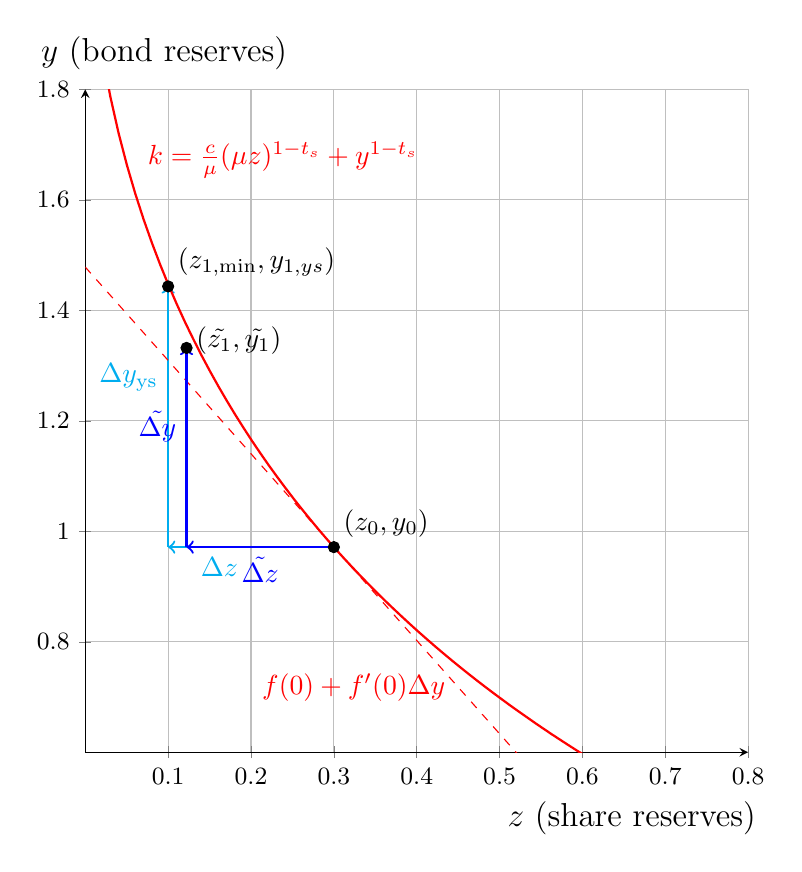
\begin{tikzpicture}
    \begin{axis}[
        xlabel={$z$ (share reserves)},
        ylabel={$y$ (bond reserves)},
        grid=major, % Adds grid lines
        axis lines=middle, % Places the axes in the middle
        width=10cm,
        height=10cm,
        xmin=0, xmax=0.8,
        ymin=0.6, ymax=1.8,
        domain=0:2,
        samples=200, % Number of sample points for smooth curve
        every axis label/.append style={font=\large}, % Makes labels larger
        ticklabel style = {font=\small},
        xlabel style={at={(ticklabel* cs:1.05)}, anchor=north, xshift=-1.9cm, yshift=-0.5cm}, % Moves xlabel outside
        ylabel style={at={(ticklabel* cs:1.05)}, anchor=south, xshift=1.0cm, yshift=-0.3cm}, % Moves ylabel outside
    ]

    % Constants & initial conditions
    \def\k{1.5}
    \def\ts{0.5}
    \def\u{1.5}
    \def\c{1.15}
    \def\phic{0.15}
    \def\phig{0.1}
    \def\zzero{0.3}
    \def\zone{0.1}
    \def\zeta{0.0001}

    % Points y0, y1
    \pgfmathsetmacro{\yzero}{( \k - \c/\u * (\u*\zzero)^(1-\ts) )^(1/(1-\ts))}
    \pgfmathsetmacro{\yone}{( \k - \c/\u * (\u*\zone)^(1-\ts) )^(1/(1-\ts))}
    % Plot points
    \addplot[only marks, mark=*] coordinates {(\zzero,\yzero) (\zone,\yone)};
    % Labels points
    \node[anchor=south west] at (axis cs:\zzero, \yzero) {$(z_0, y_0)$};
    \node[anchor=south west] at (axis cs:\zone, \yone) {$(z_{1,\text{min}}, y_{1,ys})$};
    % Show real ∆y, ∆z
    \draw[cyan, thick, ->] (axis cs:\zzero,\yzero) -- (axis cs:\zone,\yzero) node[midway, below, xshift=-0.4cm] {$\Delta z$};
    \draw[cyan, thick, ->] (axis cs:\zone,\yzero) -- (axis cs:\zone,\yone) node[midway, left, yshift=0.5cm] {$\Delta y_{\text{ys}}$};

    % YieldSpace curve in red
    \addplot[thick, red] 
        { ( \k - \c/\u * (\u * x)^(1-\ts) )^(1/(1-\ts)) };
    % Label for the yieldspace curve
    \def\labelz{0.04}
    \pgfmathsetmacro{\labely}{( \k - \c/\u * (\u*\labelz)^(1-\ts) )^(1/(1-\ts))}
    \node[anchor=north west, red, xshift=0.25cm] at (axis cs:\labelz,\labely) {$k = \frac{c}{\mu}(\mu z)^{1 - t_s} + y^{1 - t_s}$};

    % Compute spot price 'p'
    \pgfmathsetmacro{\p}{ ( (\u * (\zzero - \zeta)) / \yzero )^\ts }

    % Compute slope 'm' of the tangent line at (z0, y0)
    % m = dy/dz = 1 / (dz/dy) = 1 / (-p*/c) = -c/p*
    \pgfmathsetmacro{\m}{ -\c / \p}

    % Plot tangent line at (z0, y0)
    \addplot [dashed, red] { \yzero + \m * (x - \zzero) };
    % Label for the tangent line
    \pgfmathsetmacro{\fprimelabelx}{ 0.4 }
    \pgfmathsetmacro{\fprimelabely}{\yzero + \m * (\fprimelabelx - \zzero)}
    \node[red, xshift=-0.8cm, yshift=-0.6cm] at (axis cs:\fprimelabelx, \fprimelabely) {$f(0) + f'(0) \Delta y$};
    
    % Using the linear approximation to find ~y1
    \pgfmathsetmacro{\tildedeltay}{ (\c * (\zzero - \zeta - \zone)) / (\p - \phic * (1 - \p) * (1 - \phig))}
    \pgfmathsetmacro{\tildeyone}{\yzero + \tildedeltay}
    
    % Define and plot ~z1 for estimated ∆y
    \pgfmathsetmacro{\tildedeltaz}{\zzero - (1 / \u) * ((\u / \c) * (\k - \tildeyone^(1-\ts)))^(1 / (1-\ts)) + \phic * (1 - \p) * (1 - \phig) * (\tildedeltay / \c) }
    \pgfmathsetmacro{\tildezone}{\zzero - \tildedeltaz}
    \addplot[only marks, mark=*] coordinates {(\tildezone, \tildeyone)};
    \node[anchor=south west, yshift=-0.2cm] at (axis cs:\tildezone, \tildeyone) {$(\Tilde{z_1}, \Tilde{y_1})$};
    % Label ~∆z and ~∆y
    \draw[blue, thick, ->] (axis cs:\zzero,\yzero) -- (axis cs:\tildezone,\yzero) node[midway, below] {$\Tilde{\Delta z}$};
    \draw[blue, thick, ->] (axis cs:\tildezone,\yzero) -- (axis cs:\tildezone,\tildeyone) node[left, yshift=-1.00cm] {$\Tilde{\Delta y}$};
    
    \end{axis}
\end{tikzpicture}

\subsubsection{Refining the maximum possible short estimate}\label{newton-refinement}

Starting from the estimate in section \ref{conservative-abs-max}, we will use Newton's Method to refine our guess.
The non-linearity arising from the nested \code{max} functions in equation \eqref{pool-min-share-reserves} creates an additional challenge for refining the estimate using a gradient-base method.
We circumvent this problem by ignoring the exposure in the loss, and checking for it in an early-stopping condition during optimization.
Thus, we define the target share reserves ignoring exposure as $z_t = z_\text{min} + \text{max}(\zeta, 0)$, which is used in our loss function:

\begin{equation}\label{newton-loss}
    l(\Delta y) = z_t - z_1(\Delta y)
\end{equation}

where $z_1(\Delta y)$ is the share reserves after our current max short guess, defined in equation \eqref{reserve-after-max}.
Newton's method also requires the derivative, which we can simplify by writing in terms of the short principal derivative (Equation \eqref{eq-short-principal-derivative}) and curve fee derivative (Equation \eqref{curve-fee-derivative}).

\begin{equation}\label{delta-shares-derivative}
\begin{aligned}
    \frac{d \Delta z}{d \Delta y} &= -L^{\prime}(\Delta y)
        - \Phi^{\prime}_{\text{c,os}}(\Delta y) \cdot (1 - \phi_g) \\
    \therefore \\
    l^{\prime}(\Delta y) &= -\frac{d \Delta z}{d \Delta y} \\
\end{aligned}
\end{equation}

This gives us our Newton update:

\begin{equation}\label{newton-update}
    \Delta y_{n+1} = \Delta y_{n} - \frac{l(\Delta y_{n})}{l^{\prime}(\Delta y_{n})}
\end{equation}

\subsection{Close short}
Closing a short depends on the amount of bonds to be closed, the vault share price when opening the short, the current vault share price, the maturity time of the short, and the current time.
We first compute a normalized time remaining for the bonds:

\begin{equation}\label{normalized-time-remaining}
    \bar{T} = \frac{t_{m} - t_{c}}{d}
\end{equation}

where $t_{m}$ is the maturity time of the short, $t_c$ is the current checkpoint time, and $d$ is the bond position duration.
The pool share delta is made up of a curve component, flat component, and fee component.
The flat component is

\begin{equation}\label{close-short-flat}
    \Delta z_{\text{flat}}(\Delta y) = \frac{\Delta y}{c} \cdot (1 - \bar{T})
\end{equation}

The curve component is

\begin{equation}\label{close-short-curve}
\Delta z_{\text{curve}}(\Delta y) =
\begin{cases}
    \frac{1}{\mu} \cdot \left( \frac{\mu}{c} \cdot k - \left( y_0 - \Delta y \cdot \bar{T}^{-1} \right)^{1-t_s} \right)^{\frac{1}{1 - t_s}} - (z_{0} - \zeta) , & \text{if} \bar{T} > 0 \\
    0, & \text{otherwise}
\end{cases}
\end{equation}

The fee component is

\begin{equation}\label{close-short-fees}
\Delta z_{\text{fees}}(\Delta y) =  \frac{\Delta y}{c} \cdot \left( \phi_c \cdot (1 - p) \cdot \bar{T} + \phi_f \cdot (1 - \bar{T}) \right)
\end{equation}

Together these give the pool share delta:

\begin{equation}\label{close-short-shares-returend}
\Delta z(\Delta y) = \Delta z_{\text{flat}}(\Delta y) + \Delta z_{\text{curve}}(\Delta y) + \Delta z_{\text{fees}}(\Delta y)
\end{equation}

The amount returned to the trader is a function of this pool share delta:

\begin{equation}\label{close-short-trader-return}
    R(\Delta y) =  V(\Delta y) + \phi_f \cdot \frac{\Delta y}{c} - \Delta z(\Delta y)
\end{equation}

where $V(\Delta y)$ is defined in section \ref{trader-deposit} with the ending share price set to the share price at time of closing the short, $c_1 = c$ and $c_0$ is the share price when opening the short.
This return is only valid if the left terms, $V(\Delta y) + \phi_f \cdot \frac{\Delta y}{c}$, are greater than the pool share delta, $\Delta z$.
Otherwise, the user receives zero shares.

\subsubsection{Determining the close short bond amount from a desired return}
It could be the case where a trader wants to determine how many bonds to close to get a certain return back, in shares.
This is an intractable inverse function, much like the max short function.
However, we can follow the same procedure in sections \ref{conservative-abs-max} to produce a linear approximation of the non-linear curve pool share delta term.
Ignoring the condition where the close short returns are zero,

\begin{equation}
\begin{aligned}
    \Delta z_{\text{curve}}(\Delta y) = f(\Delta y) &= 
    \frac{1}{\mu} \cdot \left( \frac{\mu}{c} \cdot k - \left( y_0 - \Delta y \cdot \bar{T}^{-1} \right)^{1-t_s} \right)^{\frac{1}{1 - t_s}} - (z_{0} - \zeta) \\
    &\ge f(0) + f'(0) \cdot \Delta y
\end{aligned} 
\end{equation}

When we evaluate $f(\Delta y)$ at $\Delta y = 0$ we cancel the $\bar{T}$ term.
The additional terms from computing a share delta cancels out the initial effective share reserves, giving us:

\begin{equation}\label{close-short-delta-z-curve-approx}
    \Delta z_{\text{curve}}(\Delta y) \ge \Tilde{\Delta z}_{\text{curve}}(\Delta y) = - \frac{p}{c} \cdot \Delta y
\end{equation}

This was the only non-linear term, so now we can write out our full linear approximation and invert it:

\begin{equation}\label{close-short-delta-z-approx}
\begin{aligned}
    \Tilde{\Delta z}(\Delta y) &= \Delta z_{\text{flat}}(\Delta y) + \Tilde{\Delta z}_{\text{curve}}(\Delta y) + \Delta z_{\text{fees}}(\Delta y) \\
    \therefore \\
    R(\Delta y) &=  V(\Delta y) + \phi_f \cdot \tfrac{\Delta y}{c} - \Delta z(\Delta y) \\
    &\ge \tfrac{\Delta y}{c} \cdot \left( \tfrac{c_1}{c} + 2 \cdot \phi_f - \left(1 - \bar{T} \right) + p - \phi_c \cdot (1 - p) \cdot \bar{T} - \phi_f \cdot \left( 1 - \bar{T} \right) \right) \\
    \therefore \\
    \Delta y \le \Tilde{\Delta y} &= \frac{c \cdot R(\Delta y)}{\tfrac{c_1}{c} + 2 \cdot \phi_f - \left(1 - \bar{T} \right) + p - \phi_c \cdot (1 - p) \cdot \bar{T} - \phi_f \cdot \left( 1 - \bar{T} \right)}
\end{aligned}
\end{equation}

This equation allows us to conservatively approximate the amount of bonds to be shorted, $\Tilde{\Delta y}$, to provide a requested return amount to the trader, $R(\Delta y)$.
As in section \ref{newton-refinement}, we can use Newton's Method to refine the result:

\begin{equation}
\begin{aligned}
    l(\Delta y) &= R_{t}(\Delta y) - R(\Delta y) \\
    l^{\prime}(\Delta y) &= - \frac{d R(\Delta y)}{d \Delta y} \\
    R^{\prime}(\Delta y) &= V^{\prime}(\Delta Y) + \frac{\phi_f}{c} - \Delta z^{\prime}(\Delta y) \\
    \Delta z^{\prime}(\Delta y) &= \Delta z^{\prime}_{\text{curve}}(\Delta y)
    + \frac{1}{c} \cdot
    \left( \bar{T} + \phi_c \cdot (1-p) \cdot \bar{T} + \phi_f \cdot \left(1 - \bar{T}\right) \right)
\end{aligned}
\end{equation}

We will need to follow the procedure in section \ref{short-principal-derivative} to find the derivative $\Delta z^{\prime}_{\text{curve}}(\Delta y)$.
Let,

\begin{equation}
u = \frac{\mu}{c} \cdot \left( k - (y + \Delta y \cdot \bar{T})^{1-t_s} \right)
\end{equation}

\begin{equation}
\frac{du}{d \Delta y} = \frac{\mu}{c} \cdot -(1 - t_s) \cdot \bar{T} \cdot (y + \Delta y \cdot \bar{T})^{-t_s}
\end{equation}

therefore,

\begin{equation}
\begin{aligned}
\Delta z^{\prime}_{\text{curve}}(\Delta y) &= - \tfrac{1}{\mu} \cdot \tfrac{1}{1-t_s} \cdot u^{\tfrac{1}{1-t_s} - 1} \cdot \tfrac{du}{d \Delta y} \\
&= - \tfrac{1}{\mu} \cdot \tfrac{1}{1-t_s} \left( \tfrac{\mu}{c} \left( k - (y + \Delta y \cdot \bar{T})^{1 - t_s} \right) \right)^{\tfrac{t_s}{1-t_s}}
\cdot \tfrac{\mu}{c} \cdot -(1 - t_s) \cdot \bar{T} \cdot (y + \Delta y \cdot \bar{T})^{t_s} \\
&= \tfrac{\bar{T}}{c} \cdot (y + \Delta y \cdot \bar{T})^{-t_s} \cdot \left( \tfrac{\mu}{c} \cdot \left( k - (y + \Delta y \cdot \bar{T})^{1 - t_s} \right) \right)^{\tfrac{t_s}{1 - t_s}}
\end{aligned}
\end{equation}

Given these, the Newton update is the same as Equation \eqref{newton-update}.

\subsection{Targeted short}\label{targeted-short}
TODO

\section{Longs}
\subsection{Max long}

\subsubsection{The Hyperdrive-Yieldspace AMM}

For a deployed market pool, the Hyperdrive-Yieldspace AMM uses a modified \href{https://yield.is/YieldSpace.pdf}{constant power sum formula} to derive a price relationship between two assets.
In this case, our assets are vault shares, $z$, and bonds, $y$.
When base, $x$, is supplied to the market, it is converted into shares, $z$, by depositing the base into an underlying yield bearing vault.
The Hyperdrive AMM then supplies bonds, $y$, such that $k$ is kept constant.
The two are related via an invariance formula (\href{https://github.com/delvtech/hyperdrive/blob/f410574fffcb8b2556208c158494ba2972525843/crates/hyperdrive-math/src/yield_space.rs#L285}{yieldspace.rs, l285}):

\begin{equation}\label{keq}
\begin{aligned}
k &= \tfrac{\mu}{c}^{-t_{s}} x^{1 - t_{s}} + y^{1 - t_{s}} \\
&= \tfrac{c}{\mu} (\mu z)^{1 - t_{s}} + y^{1 - t_{s}}
\end{aligned}
\end{equation}

where $t_{s}$ is the time stretch constant, $c$ is the current vault share price, and $\mu$ is the share price of the vault when the Hyperdrive pool was created (aka \code{initial_share_price}).

The relationship between shares and bonds is also described using the spot price.
Our generic equation for spot price (\href{https://github.com/delvtech/hyperdrive/blob/34b562e8952cf9cf235e551484790bbc7ff65884/crates/hyperdrive-math/src/long/max.rs#L154}{max.rs, l154} and \href{https://github.com/delvtech/hyperdrive/blob/570263e2b85c411b4097132bfe7ad2a085e3180b/crates/hyperdrive-math/src/yield_space.rs#L36-L37}{yieldspace.rs, l36}) is given by:

\begin{equation}\label{simple-price}
p = \left( \tfrac{\mu z}{y} \right)^{t_s}
\end{equation}

\begin{callout}
\callouttext{bulb}{NOTE}

We can use the procedure outlined in Appendix C of the \href{https://yield.is/YieldSpace.pdf}{YieldSpace paper} to relate the price and invariant formula.
Recall from the paper:

\begin{displayquote}
In any invariant-based liquidity provision formula, the price at any point along the curve is equal to the negation of the derivative at that point

$p_{x} = -\tfrac{dy}{dx}$
\end{displayquote}

However, in Hyperdrive we consider a price that is $<=1$, while the YieldSpace paper assumes it is $>=1$, which we can express as an inversion:
$p_{\text{hyperdrive}} = \tfrac{1}{p_{\text{yieldspace}}}$.
Given this, and that base is converted to shares via $x = cz$, we can derive the invariant from the price as such:

\begin{displaymath}
\begin{aligned}
-\tfrac{dy}{dx} &= p^{-1} \\
-\tfrac{dy}{dx} &= \left( \tfrac{\mu z}{y} \right)^{-t_s} \\
-\tfrac{dy}{dx} &= \left( \mu \tfrac{x}{c} \right)^{-t_s} y^{t_{s}} \\
-y^{-t_{s}} \tfrac{dy}{dx} &= \left( \mu \tfrac{x}{c} \right)^{-t_s} \\
-\int{y^{-t_{s}}}{dy} &= \int{\left( \mu \tfrac{x}{c} \right)^{-t_s}}{dx} \\
-\tfrac{1}{1-t_{s}} y^{1 - t_{s}} + \alpha_{1} &= \mu^{-t_{s}} \tfrac{1}{c^{-t_{s}}} \left( \tfrac{1}{1-t_{s}} x^{1-t_{s}} + \alpha_{2} \right) \\
-y^{1 - t_{s}} + \alpha_{1}^{\prime} &= \left( \tfrac{\mu}{c} \right)^{-t_{s}} x^{1-t_{s}} + \alpha_{2}^{\prime\prime} \\
\alpha_{1}^{\prime} - \alpha_{2}^{\prime\prime} &= \left( \tfrac{\mu}{c} \right)^{-t_{s}} x^{1 - t_{s}} + y^{1 - t_{s}} \\
k &= \tfrac{c}{\mu} \left( \tfrac{\mu}{c} \right)^{1 - t_{s}} x^{1 - t_{s}} + y^{1 - t_{s}} \\
k &= \tfrac{c}{\mu} \left( \tfrac{\mu}{c} x \right)^{1 - t_{s}} + y^{1 - t_{s}} \\
k &= \tfrac{c}{\mu} (\mu z)^{1 - t_{s}} + y^{1 - t_{s}} \\
\end{aligned}
\end{displaymath}

\end{callout}

Hyperdrive computes fees that are removed from the system whenever a trade is made.
The fee constants are denoted with $\phi$, where $\phi_{f}$ refers to the flat fee, $\phi_{c}$ refers to the curve fee, and $\phi_{g}$ is the governance fee.
The open-long governance and curve fees can be written as a function of the base transferred, $\Delta x$, and initial spot price (\href{https://github.com/delvtech/hyperdrive/blob/2a8c81fa401f31031be8ad87117a0a7a85a866ff/crates/hyperdrive-math/src/long/fees.rs}{fees.rs}):

\begin{align}
\label{curve-fee} \Phi_{c}(\Delta x) &= \phi_{c} \left( \tfrac{1}{p_{0}} - 1 \right) \Delta x \\
\label{gov-fee} \Phi_{g}(\Delta x) &= \phi_{g} p_{0} \Phi_{c}(\Delta x) = \phi_{g} \phi_{c} \left( 1 - p_{0} \right) \Delta x
\end{align}

where $p_{0}$ is the spot price before the trade, i.e. the current spot price.
We do not include a function for the flat fee because it is only applied when closing a long.

\begin{callout}
\callouttext{bulb}{NOTE}

We will use capital letters to denote functions and lower-case letters to denote scalars.
\end{callout}

The pool's maximum spot price such that the trade doesn't result in negative interest is given by (\href{https://github.com/delvtech/hyperdrive/blob/570263e2b85c411b4097132bfe7ad2a085e3180b/crates/hyperdrive-math/src/long/max.rs#L147}{max.rs, line 147} and derived in \href{https://github.com/delvtech/hyperdrive/issues/655}{issue \#655}):

\begin{equation}\label{pmax}
p_{\text{max}} = \tfrac{(1 - \phi_{f})}{1 + \phi_{c} \left( \tfrac{1}{p_{0}}-1 \right)(1-\phi_{f})}
\end{equation}

\subsubsection{Deriving the target base and bond amounts}

Our goal is to determine the maximum long that can be opened for a given market, which will result in the max spot price.
The two price equations can be used to derive the target reserve levels for a pool with the max spot price.
These are given as target shares, $z_{t}$, and target bonds, $y_{t}$.
First we will solve for the target bond reserves in terms of the target share reserves by setting equations \eqref{simple-price} and \eqref{pmax} to be equal \href{https://github.com/delvtech/hyperdrive/blob/570263e2b85c411b4097132bfe7ad2a085e3180b/crates/hyperdrive-math/src/long/max.rs#L162}{max.rs, l162}:

\begin{equation}
\begin{aligned}
p &= p_{\text{max}} \\
\left( \tfrac{\mu z_{t}}{y_{t}} \right)^{T_s} &= \tfrac{(1 - \phi_{f})}{1 + \phi_{c} \left( \tfrac{1}{p_{0}}-1 \right)(1-\phi_{f})} \\
\tfrac{\mu z_{t}}{y_{t}} &= \left( \tfrac{\left( 1 - \phi_{f} \right)}{1 + \phi_{c} \left( \tfrac{1}{p_{0}}-1 \right) \left( 1-\phi_{f} \right)} \right)^{\tfrac{1}{t_{s}}} \\
y_{t} &= \tfrac{\mu z_{t}}{\left( \tfrac{(1 - \phi_{f})}{1 + \phi_{c} \left( \tfrac{1}{p_{0}}-1 \right)(1-\phi_{f})} \right)^{\tfrac{1}{t_{s}}}} \\
y_{t} &= \mu z_{t} \left( \tfrac{1 + \phi_{c} (\tfrac{1}{p_{0}} - 1) (1 - \phi_{f})}{1 - \phi_{f}} \right)^{\tfrac{1}{t_{s}}}
\end{aligned}
\end{equation}

\begin{callout}
\callouttext{bulb}{NOTE}
That last step required some algebra acrobatics:
\begin{displaymath}
\tfrac{1}{\left( \cfrac{x}{y} \right)^{c}} = \tfrac{1}{\cfrac{x^c}{y^c}} = \tfrac{1}{\cfrac{y^{-c}}{x^{-c}}} = \tfrac{1}{\left( \cfrac{y}{x} \right)^{-c}} = \left( \tfrac{y}{x} \right)^{c}
\end{displaymath}
\end{callout}

Using the invariant equation we can solve for $z_{t}$ isolated, without $y_{t}$ \href{https://github.com/delvtech/hyperdrive/blob/570263e2b85c411b4097132bfe7ad2a085e3180b/crates/hyperdrive-math/src/long/max.rs#L175}{max.rs, l175}:

\begin{equation}
\begin{aligned}
k &= \tfrac{c}{\mu} (\mu z_{t})^{1 - t_{s}} + y_{t}^{1 - t_{s}} \\
k &= \tfrac{c}{\mu} (\mu z_{t})^{1-t_{s}} + \left( \mu z_{t} \left( \tfrac{1 + \phi_{c} (\tfrac{1}{p_{0}}-1) (1 - \phi_{f})}{1 - \phi_{f}} \right)^{\tfrac{1}{t_{s}}} \right)^{1-t_{s}} \\
k &= \left( \mu z_{t} \right)^{1 - t_{s}} \left( \tfrac{c}{\mu} + \left( \tfrac{1 + \phi_{c}\left( \tfrac{1}{p_{0}} - 1 \right) \left( 1 - \phi_{f} \right)}{1 - \phi_{f}} \right)^{\tfrac{1-t_{s}}{t_{s}}} \right) \\
\left( \mu z_{t} \right)^{1-t_{s}} &= k \bigg/ \left( \tfrac{c}{\mu} + \left( \tfrac{1 + \phi_{c}\left( \tfrac{1}{p_{0}} - 1 \right) \left( 1 - \phi_{f} \right)}{1 - \phi_{f}} \right)^{\tfrac{1-t_{s}}{t_{s}}} \right) \\
\mu z_{t} &= \left( k \bigg/ \left( \tfrac{c}{\mu} + \left( \tfrac{1 + \phi_{c}\left( \tfrac{1}{p_{0}} - 1 \right) \left( 1 - \phi_{f} \right)}{1 - \phi_{f}} \right)^{\tfrac{1-t_{s}}{t_{s}}} \right) \right)^{\tfrac{1}{1-t_{s}}} \\
z_{t} &= \tfrac{1}{\mu} \left( k \bigg/ \left( \tfrac{c}{\mu} + \left( \tfrac{1 + \phi_{c} \left( \tfrac{1}{p_{0}} - 1 \right) \left( 1 - \phi_{f} \right)}{1 - \phi_{f}} \right)^{\tfrac{1-t_{s}}{t_{s}}} \right) \right)^{\tfrac{1}{1 - t_{s}}}
\end{aligned}
\end{equation}

Next, we plug this result into our earlier equation to get $y_{t}$ isolated (\href{https://github.com/delvtech/hyperdrive/blob/570263e2b85c411b4097132bfe7ad2a085e3180b/crates/hyperdrive-math/src/long/max.rs#L202}{max.rs, l202}):

\begin{equation}\label{yt-price}
\begin{aligned}
y_{t} &= \mu z_{t} \left( \tfrac{1 + \phi_{c} (\tfrac{1}{p_{0}} - 1) (1 - \phi_{f})}{1 - \phi_{f}} \right)^{\tfrac{1}{t_{s}}} \\
&= \left( k \bigg/ \left( \tfrac{c}{\mu} + \left( \tfrac{1 + \phi_{c} \left( \tfrac{1}{p_{0}} - 1 \right) \left( 1 - \phi_{f} \right)}{1 - \phi_{f}} \right)^{\tfrac{1-t_{s}}{t_{s}}} \right) \right)^{\tfrac{1}{1 - t_{s}}} \left( \tfrac{1 + \phi_{c} \left( \tfrac{1}{p_{0}} - 1 \right) \left( 1 - \phi_{f} \right)}{1 - \phi_{f}} \right)^{\tfrac{1}{t_{s}}} \\
\end{aligned}
\end{equation}

These target reserve levels then correspond to opening a long for a delta base or bonds (\href{https://github.com/delvtech/hyperdrive/blob/f410574fffcb8b2556208c158494ba2972525843/crates/hyperdrive-math/src/long/max.rs#L207}{max.rs, l213} and \href{https://github.com/delvtech/hyperdrive/blob/f410574fffcb8b2556208c158494ba2972525843/crates/hyperdrive-math/src/long/max.rs#L213}{max.rs, l219}, respectively):

\begin{align}
\Delta x &= c (z_{t} - z) \label{dx} \\
\Delta y &= (y - y_{t}) - \Phi_{c}(\Delta x) \label{dy}
\end{align}

If the pool is solvent after opening this long, then we're done.
Otherwise, we will use a numerical approach to estimate the actual trade amount.

\subsubsection{Iterative refinement of the maximum long amount}

Opening a long causes a change in both base and bonds and is impacted by fees.
Without a closed-form solution, we will need a numerical approach to estimate the actual trade amount for most pool conditions.
Specifically, we will use Newton's method with the pool's solvency as our objective function.
Solvency captures the protocol's ability to pay its debts by measuring its assets versus its liabilities and minimum reserves.
Assets are the share reserves, $z$.
Liabilities are the aggregate long exposure.
Minimum share reserves are set in a pool's configuration, as $z_{\text{min}}$.
Liabilities and reserves are converted to common units (base or shares) via the share price, $c$.

\begin{equation}\label{solvency}
\begin{aligned}
S(z) &= \text{assets} - \text{liabilities} - \text{minimum\_reserves} \\
&= z - \tfrac{l}{c} - z_{\text{min}} \\
&= \tfrac{1}{c} \left( x - l - x_{\text{min}} \right)
\end{aligned}
\end{equation}

For a single long, the change in exposure is given by the amount of bonds returned, $\Delta l = Y(\Delta x)$ (aka the amount of longs opened, or long amount).
The amount of bonds returned can be broken down into a component without fees and a fee component (\href{https://github.com/delvtech/hyperdrive/blob/f410574fffcb8b2556208c158494ba2972525843/crates/hyperdrive-math/src/long/open.rs#L11}{open.rs, l11}):

\begin{equation}\label{long-amount}
Y(\Delta x) = Y_{*}(\Delta x) - \Phi_{c}(\Delta x)
\end{equation}

where, for some initial bond reserves, $y_{0}$, and base reserves, $x_{0}$ (or alternatively initial \href{https://github.com/delvtech/hyperdrive/blob/34b562e8952cf9cf235e551484790bbc7ff65884/contracts/src/libraries/HyperdriveMath.sol#L147}{effective share reserves}, $z_{0}$),

\begin{equation}
\begin{aligned}
Y_{*}(\Delta x) &= y_{0} - \left( k - \tfrac{c}{\mu} \left( \mu \left( z_{0} + \tfrac{\Delta x}{c} \right) \right)^{1 - t_{s}} \right)^{\tfrac{1}{1 - t_{s}}} \\
&= y_{0} - \left( k - \tfrac{c}{\mu} \left( \tfrac{\mu}{c} \left( x_{0} + \Delta x \right) \right)^{1 - t_{s}} \right)^{\tfrac{1}{1 - t_{s}}} \\
&= y_{0} - \left( k - \left( \tfrac{\mu}{c} \right)^{- t_{s}} \left( x_{0} + \Delta x \right)^{1 - t_{s}} \right)^{\tfrac{1}{1 - t_{s}}} \\
\end{aligned}
\end{equation}

When a long is opened, the share reserves is increased by (\href{https://github.com/delvtech/hyperdrive/blob/f410574fffcb8b2556208c158494ba2972525843/crates/hyperdrive-math/src/long/max.rs#L315}{max.rs, l315}):

\begin{equation}\label{dz}
\Delta z = \tfrac{\Delta x - \Phi_{g}(\Delta x)}{c}
\end{equation}

Using these components, we can derive our objective function as the solvency after a change in shares (\href{https://github.com/delvtech/hyperdrive/blob/f410574fffcb8b2556208c158494ba2972525843/crates/hyperdrive-math/src/long/max.rs#L329}{max.rs, l329}):

\begin{equation}
\begin{aligned}
S(\Delta z) &= \left( z_{0} + \Delta z \right) - \left( \tfrac{l_{0} + l_{\text{chk}} + \Delta l}{c} \right) - z_{\text{min}} \\
\therefore \\
S(\Delta x) &= \tfrac{1}{c} \left( x_{0} + \Delta x - \Phi_{g}\left( \Delta x \right) - l_{0} - l_{\text{chk}} - Y(\Delta x) - x_{\text{min}} \right) \\
\end{aligned}
\end{equation}

where $l_{\text{chk}}$ is the checkpoint long exposure and is assumed to be $>= 0$.
We add the checkpoint exposure to account for negative exposure from non-netted shorts in the checkpoint.
We will keep everything in units of base, but see \href{https://github.com/delvtech/hyperdrive/blob/f410574fffcb8b2556208c158494ba2972525843/crates/hyperdrive-math/src/long/max.rs#L336}{max.rs, l336} for the implementation using units of shares.

In summary, our optimization objective is

\begin{equation}
\begin{split}
\argmax\limits_{\Delta x} -S(\Delta x) \\
\text{s.t.} S(\Delta x) > 0
\end{split}
\end{equation}


To perform Newton's method we also need the gradient of the objective, starting with the long amount:

\begin{equation}\label{long-amount-no-fees}
Y^{\prime}(\Delta x) = Y_{*}^{\prime}(\Delta x) - \Phi_{c}^{\prime}(\Delta x)
\end{equation}

where,

\begin{equation}
\begin{aligned}
Y_{*}^{\prime}(\Delta x) &= \left( \tfrac{\mu}{c} \right)^{-t_{s}} \left( x_{0} + \Delta x \right)^{-t_{s}} \left( k - \left( \tfrac{\mu}{c} \right)^{-t_{s}} \left( x_{0} + \Delta x \right)^{1-t_{s}}  \right)^{\tfrac{t_{s}}{1-t_{s}}} \\
&= \left( \mu (z_{0} + \tfrac{\Delta x}{c}) \right)^{-t_{s}} \left( k - \tfrac{c}{\mu} \left( \mu (z_{0} + \tfrac{\Delta x}{c} \right)^{1 - t_{s}} \right)^{\tfrac{t_{s}}{1 - t_{s}}} \\
\end{aligned}
\end{equation}

We also need the gradient of the governance and curve fee calculations:

\begin{align}
\Phi_{c}^{\prime}(\Delta x) &= \phi_{c}(\tfrac{1}{p_{0}} - 1) \\
\Phi_{g}^{\prime}(\Delta x) &= \phi_{g}p_{0}\Phi_{c}^{\prime}(\Delta x)
\end{align}

Together, these give us the solvency gradient:

\begin{equation}
\begin{aligned}
S^{\prime}(\Delta x) &= \tfrac{1}{c} \left( 1 - \Phi_{g}^{\prime}(\Delta x) - Y^{\prime}(\Delta x) \right) \\
\end{aligned}
\end{equation}

We want to discover a $\Delta x$ to push the pool to be as close to insolvent as possible, without passing over to actually being insolvent.
We achieve this by maximizing the negative solvency, since solvency decreases as more longs are opened.
For each iteration of Newton's method (\href{https://github.com/delvtech/hyperdrive/blob/f410574fffcb8b2556208c158494ba2972525843/crates/hyperdrive-math/src/long/max.rs#L73}{max.rs, l73}):

\begin{equation}
\begin{aligned}
\Delta x_{n+1} &= \Delta x_n - \tfrac{S(\Delta x_n)}{S'(\Delta x_n)} \\
&= \Delta x_n + \tfrac{S(\Delta x_n)}{-S'(\Delta x_n)}
\end{aligned}
\end{equation}

In the actual implementation, we will iteratively compute solvency for the new $\Delta x_{n}$ until the system is no longer solvent, and then back up one step to return the maximum long.

\subsubsection{Deriving an initial guess for the max long amount}

The rate of convergence for Newton's method is improved with a better initial guess, $\Delta x_{n=0}$.
To derive an initial guess, we can use a conservative price estimate, $p_{r}$, to approximate $Y(\Delta x)$ (\href{https://github.com/delvtech/hyperdrive/blob/f410574fffcb8b2556208c158494ba2972525843/crates/hyperdrive-math/src/long/max.rs#L253}{max.rs, l253}):

\begin{equation}\label{approx-long-amount}
\begin{aligned}
Y(\Delta x) &\approx \tfrac{\Delta x}{p_{r}} - \Phi_{c}(\Delta x) \\
&\approx \Delta x \left( \tfrac{1}{p_{r}} - \phi_{c} \left( \tfrac{1}{p_{0}} - 1 \right) \right) \\
\end{aligned}
\end{equation}

We define our initial solvency as in equation \eqref{solvency}:
$s_{0} = \tfrac{1}{c} \left(x_{0} - l_{0} - x_{\text{min}} \right)$.
Plugging this into our solvency function $S(\Delta x)$, we can calculate the share reserves and exposure after opening a long with $\Delta x$ base as (\href{https://github.com/delvtech/hyperdrive/blob/f410574fffcb8b2556208c158494ba2972525843/crates/hyperdrive-math/src/long/max.rs#L259}{max.rs, l259}):

\begin{equation}
\begin{aligned}
Z(\Delta x) &= z_0 + \tfrac{\Delta x - \Phi_{g}(\Delta x)}{c} \\
Z(\Delta x) &= \tfrac{1}{c} \left( x_0 + \Delta x - \Phi_{g}(\Delta x) \right) \\
\end{aligned}
\end{equation}

\begin{equation}
\begin{aligned}
L(\Delta x) &= l_0 + l_{\text{chk}} + 2 Y(\Delta x) - \Delta x + \Phi_{g}(\Delta x) \\
&= l_0 + l_{\text{chk}} + 2 p_{r}^{-1} \Delta x - 2 \Phi_{c}(\Delta x) - \Delta x + \Phi_{g}(\Delta x)
\end{aligned}
\end{equation}

These formulae allow us to calculate the approximate ending solvency of (\href{https://github.com/delvtech/hyperdrive/blob/f410574fffcb8b2556208c158494ba2972525843/crates/hyperdrive-math/src/long/max.rs#L271}{max.rs, l271}):

\begin{equation}
\begin{aligned}
S(\Delta x) &\approx Z(\Delta x) - \tfrac{L(\Delta x)}{c} - z_{\text{min}} \\
&\approx \tfrac{1}{c} \left( x_0 + \Delta x - \Phi_{g}(\Delta x) - L(\Delta x) - x_{\text{min}} \right) \\
&\approx \tfrac{1}{c} \left( x_0 + 2 \Delta x - 2 \Phi_{g}(\Delta x) - l_{0} - l_{\text{chk}} - 2\tilde{Y}(\Delta x) - x_{\text{min}} \right) \\
\end{aligned}
\end{equation}

If we rearrange to represent the initial solvency, $s_0$, then we can solve for $\Delta x$ (\href{https://github.com/delvtech/hyperdrive/blob/f410574fffcb8b2556208c158494ba2972525843/crates/hyperdrive-math/src/long/max.rs#L278}{max.rs, l278}):

\begin{equation}\label{approx-solvency}
\begin{aligned}
s_{0} - \tfrac{1}{c} l_{\text{chk}} + \tfrac{2}{c} \left( \Delta x - \Phi_{g}(\Delta x) - \tilde{Y}(\Delta x) \right) &\approx 0 \\
s_{0} - \tfrac{1}{c} l_{\text{chk}} + \tfrac{2}{c} \left( \Delta x - \Phi_{g}(\Delta x) - \tilde{Y}(\Delta x) \right) &\approx 0 \\
s_{0} - \tfrac{1}{c} l_{\text{chk}} + \tfrac{2}{c} \Delta x \left( 1 - \phi_{g}\phi_{c} \left( 1 - p_{0} \right) - \tfrac{1}{p_{r}} + \phi_{c} \left( \tfrac{1}{p_{0}} - 1 \right) \right) &\approx 0 \\
\end{aligned}
\end{equation}

\begin{equation}
\begin{aligned}
&\therefore \\
\Delta x &\approx \tfrac{c}{2} \tfrac{-(s_{0}-(\tfrac{1}{c} l_{\text{chk}}))}{1 - \phi_{g}\phi_{c} \left( 1 - p_{0} \right) - p_{r}^{-1} + \phi_{c} \left( p_{0}^{-1} - 1 \right)} \\
\Delta x &\approx \tfrac{c}{2} \tfrac{s_{0} + \tfrac{1}{c} l_{\text{chk}}}{p_{r}^{-1} + \phi_{g}\phi_{c} \left( 1 - p_{0} \right) - \phi_{c} \left( p_{0}^{-1} - 1 \right) - 1} \\
\end{aligned}
\end{equation}

This gives us the initial value for $\Delta x_{0}$ in the iterative process.

\begin{callout}
\callouttext{exclamation}{Discrepancy}

This does not match \href{https://github.com/delvtech/hyperdrive/blob/5c12ca877c7dec2da03fac2e033141db8cfeb099/crates/hyperdrive-math/src/long/max.rs#L73}{max.rs, l73}, which has the numerator equal to $s_{0} + l_{\text{chk}}$.

\end{callout}


\subsection{Targeted long}

\subsubsection{Targeted long for a given rate}

We can follow a similar derivation to get a long that results in a \textit{target} fixed rate (aka spot rate). The fixed rate for a Hyperdrive pool given the spot price, $p$, and the annualized position duration, $t_{d}$ is given by:

\begin{equation}
r = (1-p)(p t_{d})^{-1}
\end{equation}

Note that the conversion from a ``price'' (which is computed at a single point in time) to a ``rate'' (which is computed using at least 2 points in time) is automatic because of the predetermined position duration.
Solving for $p$, we get:

\begin{equation}
\begin{aligned}
(1-p)(p t_{d})^{-1} &= r \\
\tfrac{1}{p t_{d}} - \tfrac{1}{t_{d}} &= r \\
\tfrac{1}{p} \tfrac{1}{t_{d}}  &= r + \tfrac{1}{t_{d}} \\
\tfrac{1}{p} &= t_{d} \left( r + \tfrac{1}{t_{d}} \right) \\
p &= \left( rt_{d} + 1 \right)^{-1}
\end{aligned}
\end{equation}

As before, we use $p = \left( \tfrac{\mu z_{t}}{y_{t}} \right)^{t_{s}}$ to find target reserve bonds, $y_{t}$, in terms of a target rate, $r_{t}$ (\href{https://github.com/delvtech/hyperdrive/blob/f410574fffcb8b2556208c158494ba2972525843/crates/hyperdrive-math/src/utils.rs#L112}{utils.rs, l112}):

\begin{equation}\label{yt-zt-rate}
\begin{aligned}
\left( \tfrac{\mu z_t}{y_t} \right)^{t_s} &= \tfrac{1}{r t_d + 1} \\
\tfrac{\mu z_t}{y_t} &= \left( \tfrac{1}{r t_d + 1} \right)^{\tfrac{1}{t_s}} \\
y_t &= \tfrac{\mu z_t}{\left( \tfrac{1}{r t_d + 1} \right)^{\tfrac{1}{t_s}}} \\
y_t &= \mu z_t \left( r t_d + 1 \right)^{\tfrac{1}{t_s}}
\end{aligned}
\end{equation}

We then use the invariant formula from Equation \eqref{keq} to determine the share reserves required for a given rate.

\begin{equation}
\begin{aligned}
\tfrac{c}{\mu} (\mu z_{t})^{1 - t_{s}} + y_{t}^{1 - t_{s}} &= k \\
\tfrac{c}{\mu} (\mu z_{t})^{1 - t_{s}} + \left( \mu z_{t} \left( r_{t}t_{d}+1 \right)^{\tfrac{1}{t_{s}}} \right)^{1 - t_{s}} &= k \\
\tfrac{c}{\mu} (\mu z_{t})^{1 - t_{s}} + \left( \mu z_{t} \right)^{1-t_{s}} \left( \left( r_{t}t_{d}+1 \right)^{\tfrac{1}{t_{s}}} \right)^{1 - t_{s}} &= k \\
(\mu z_{t})^{1 - t_{s}} \left( \tfrac{c}{\mu} +  \left( (r_{t} t_{d}+1)^{\tfrac{1}{t_{s}}} \right)^{1-t_{s}} \right) &= k \\
(\mu z_{t})^{1 - t_{s}} &=  \tfrac{k}{ \tfrac{c}{\mu} + \left( (r_{t} t_{d}+1)^{\tfrac{1}{t_{s}}} \right)^{1-t_{s}}} \\
z_{t} &= \tfrac{1}{\mu} \left( \tfrac{k}{ \tfrac{c}{\mu} + \left( (r_{t} t_{d}+1)^{\tfrac{1}{t_{s}}} \right)^{1-t_{s}}} \right)^{\tfrac{1}{1-t_{s}}}
\end{aligned}
\end{equation}

And finally, we plug this in to equation \eqref{yt-zt-rate} to isolate the target bonds, $y_{t}$.

\begin{equation}
y_{t} = \left( \tfrac{k}{ \tfrac{c}{\mu} +  \left( \left( r_{t} t_{d} + 1 \right)^{\tfrac{1}{t_{s}}} \right)^{1-t_{s}}} \right)^{1-t_{s}} \left( r_{t} t_{d} + 1 \right)^{\tfrac{1}{t_{s}}}
\end{equation}

Using these targets in Equations \eqref{dx} and \eqref{dy}, we can compute the long base amount to hit a target rate assuming an infinitesimally-derived price (i.e. spot price).
The approximate reserve levels for a target rate are much more likely to be solvent than the reserves after an approximated maximum long, but we still have to deal with the discrepancy between the spot price and the realized price that arises from a realistic trade size.

\subsubsection{Iteratively finding a trade for a target rate}

We need to know how the rate changes when base reserves change, $R(\Delta x)$, which will become our new objective function.
The derivative of this objective will give us the updates in each step of the refinement algorithm.

Picking up from \eqref{long-amount}, we can write the full equation for the bonds received for a given base provided from a long trade (\href{https://github.com/delvtech/hyperdrive/blob/c167ab4b35722388c3d75ac012cbb262cba00a77/crates/hyperdrive-math/src/long/open.rs#L12}{open.rs, l112}):

\begin{equation}
    Y(\Delta x) = y_{0} - \left( k - \left( \tfrac{\mu}{c} \right)^{- t_{s}} \left( x_{0} + \Delta x \right)^{1 - t_{s}} \right)^{\tfrac{1}{1 - t_{s}}} - \phi_{c} \left( \tfrac{1}{p_{0}} - 1 \right) \Delta x
\end{equation}

This is also the amount that is subtracted from the pool, i.e. $\Delta y_{\text{pool}} = Y(\Delta x)$ and thus $y_{\text{new-pool}} = y_{\text{old-pool}} - Y(\Delta x)$.
The corresponding delta that would be applied to the pool's effective share reserves is (\href{https://github.com/delvtech/hyperdrive/blob/c167ab4b35722388c3d75ac012cbb262cba00a77/crates/hyperdrive-math/src/long/open.rs#L63}{open.rs, l63}):

\begin{equation}
\begin{aligned}
\Delta z_{e, \text{pool}} &= \tfrac{1}{c} \left( \Delta x - \Phi_{g}(\Delta x) \right) - \zeta \\
&= \tfrac{\Delta x}{c} \left( 1 - \phi_{g} \phi_{c} \left( 1 - p_{0} \right) \right) - \zeta
\end{aligned}
\end{equation}

where $\zeta$ is the pool's zeta adjustment state, which is unchanged when opening positions.
The instantaneous spot price given pool reserve levels $(z_{e}, y)$ is

\begin{equation}
p = \left( \tfrac{\mu z_{e}}{y} \right)^{t_{s}}
\end{equation}

Together these allow us to derive the new share price after opening a long (\href{https://github.com/delvtech/hyperdrive/blob/18dfd4aa5a7f8d19bd34d9693aadf773995b1b14/crates/hyperdrive-math/src/long/open.rs#L52}{open.rs, l52}):

\begin{equation}
\begin{aligned}
P(\Delta x) &= \left( \tfrac{\mu \left( z_{e0, \text{pool}} + \Delta z_{e, \text{pool}} \right)}{\left( y - \Delta y_{\text{pool}} \right)} \right)^{t_{s}} \\
&= \left( \tfrac{\mu \left( z_{e0} + \tfrac{\Delta x}{c} \left( 1 - \phi_{g} \phi_{c} \left( 1 - p_{0} \right) \right) - \zeta \right)}{\left( y_{0} - \left( y_{0} - \left( k - \left( \tfrac{\mu}{c} \right)^{- t_{s}} \left( x_{0} + \Delta x \right)^{1 - t_{s}} \right)^{\tfrac{1}{1 - t_{s}}} - \phi_{c} \left( \tfrac{1}{p_{0}} - 1 \right) \Delta x \right) \right)} \right)^{t_{s}} \\
\end{aligned}
\end{equation}

where again $p_{0}$, $y_{0}$, $z_{e0}$, and $x_{0}$ are the spot price, bond reserves, effective share reserves, and base reserves before the trade, respectively.

We will also need the derivative of this function:

\begin{multline}
P^{\prime}(\Delta x) = t_{s} \left( \frac{y_{0} - Y(\Delta x)}{\mu \left( z_{e0} + \tfrac{\Delta x}{c} - \tfrac{\Phi_{g}(\Delta x)}{c} - \zeta \right)} \right)^{1 - t_{s}} \\
\frac{ \left( y_{0} - Y(\Delta x) \right) \tfrac{\mu}{c} \left( 1 - \Phi^{\prime}_{g}(\Delta x) \right) + Y^{\prime}(\Delta x) \mu \left( z_{e0} + \tfrac{\Delta x}{c} - \tfrac{\Phi_{g}(\Delta x)}{c} - \zeta \right)}{\left( y_{0} - Y(\Delta x) \right)^{2}}
\end{multline}

Given this, we can write the rate:

\begin{equation}
R(\Delta x) = \left( 1 - P(\Delta x) \right) \left( P(\Delta x) t_{d} \right)^{-1}
\end{equation}

And the derivative of the rate:

\begin{equation}
\begin{aligned}
R^{\prime}(\Delta x) &= \frac{-P^{\prime}(\Delta x) P(\Delta x) t_{d} - \left( 1 - P(\Delta x) \right) \left( P^{\prime}(\Delta x) t_{d} \right)}{(P(\Delta x) t_{d})^{2}} \\
&= \frac{-P^{\prime}(\Delta x) P(\Delta x) t_{d} - P^{\prime}(\Delta x) t_{d} + P^{\prime}(\Delta x) P(\Delta x) t_{d}}{(P(\Delta x) t_{d})^{2}} \\
&= \frac{-P^{\prime}(\Delta x)}{P(\Delta x)^2 t_{d}}
\end{aligned}
\end{equation}

We can now write our optimization function for the Newton updates.
$l(\Delta x) = R(\Delta x) - r_{t}$ shifts the trading curve down towards the zero-point.

\begin{equation}
\begin{split}
\argmax\limits_{\Delta x} (R(\Delta x) - r_{t}) \\
\text{s.t.} S(\Delta x) > 0
\end{split}
\end{equation}

As before, the derivative of loss gives us our $\Delta x$:

\begin{equation}
\begin{aligned}
\Delta x_{n+1} &= \Delta x - \frac{l(\Delta x)}{l^{\prime}(\Delta x)} \\
&= \Delta x_{n} - \frac{R(\Delta x) - r_{t}}{R^{\prime}(\Delta x)} \\
&= \Delta x_{n} + \frac{R(\Delta x) - r_{t}}{-R^{\prime}(\Delta x)}
\end{aligned}
\end{equation}

\pagebreak 

The derivative of the price after a long.

The price after a long that moves shares by $\Delta z$ and bonds by $\Delta y$
is equal to

\begin{equation}
p(\Delta z) = \left( \frac{\mu \cdot
    (z_{0} + \Delta z - (\zeta_{0} + \Delta \zeta))}
    {y - \Delta y} \right)^{t_{s}}
\end{equation}

where $t_{s}$ is the time stretch constant and $z_{0}$ is the initial
share reserves, and $\zeta$ is the zeta adjustment.
The zeta adjustment is constant when opening a long, i.e.
$\Delta \zeta = 0$, so we drop the subscript. Equivalently, for some
amount of \code{delta_base}$= \Delta x$ provided to open a long, we can write:

\begin{equation}
p(\Delta x) = \left(
    \frac{\mu (z_{0} + \frac{1}{c}
    \cdot \left( \Delta x - \Phi_{g}(\Delta x) \right) - \zeta)}
    {y_0 - y(\Delta x)}
\right)^{t_{s}}
\end{equation}

where $\Phi_{g}(\Delta x)$ is the \code{open_long_governance_fee} (Eq \eqref{gov-fee}),
$y(\Delta x)$ is the \code{long_amount},

In other words,

\begin{equation}
z_1 = z_0 + \frac{
    \Delta x - \phi_g \phi_c \left( 1 - p \right) \Delta x
}{c}
\end{equation}

and $z_{e,1} = z_{1} - \zeta$. Therefore,

\begin{equation}
z_{e,1} = z_0 + \frac{
    \Delta x - \phi_g \phi_n \left( 1 - p \right) \Delta x
}{c} - \zeta
\end{equation}

and

\begin{equation}
p(\Delta x) = \left( \frac{\mu z_{e,1}}{y_{0} - y(x)} \right)^{t_{s}}
\end{equation}

To compute the derivative, we first define some auxiliary variables:

\begin{equation}
\begin{aligned}
a(\Delta x) &= \mu (z_{0} + \frac{\Delta x}{c} - \frac{\Phi_{g}(\Delta x)}{c} - \zeta) \\
&= \mu \left( z_{e,0} + \frac{\Delta x}{c} - \frac{\Phi_{g}(\Delta x)}{c} \right) \\
b(\Delta x) &= y_0 - y(\Delta x) \\
v(\Delta x) &= \frac{a(\Delta x)}{b(\Delta x)}
\end{aligned}
\end{equation}

and thus $p(\Delta x) = v(\Delta x)^{t_{s}}$.
Given these, we can write out intermediate derivatives:

\begin{equation}
\begin{aligned}
a'(\Delta x) &= \frac{\mu}{c} (1 - \Phi_{g}'(\Delta x)) \\
b'(\Delta x) &= -y'(\Delta x) \\
v'(\Delta x) &= \frac{b(\Delta x) a'(\Delta x) - a(\Delta x) b'(\Delta x)}{b(\Delta x)^2}
\end{aligned}
\end{equation}

And finally, the price after long derivative is:

\begin{equation}
p'(\Delta x) = v'(\Delta x) t_{s} v(\Delta x)^{(t_{s} - 1)}
\end{equation}

\section{Liquidity}
TODO

\end{document}
